\newpage

\part*{Appendices}

\section{Implementation details of Cal-QL}
Our algorithm, \methodname\ is illustrated in Algorithm~\ref{alg:practical_alg}. A complete implementation of the functions in python-style is provided in Appendix~\ref{app:calql_algo}.

\subsection{\methodname\ Algorithm}
We use $J_Q(\theta)$ to denote the calibrated conservative regularizer for the Q network update:
\begin{align}
    \label{eqn:calql_training_J}
    J_Q(\theta):=&\;{{\alpha \underbrace{\left(\mathbb{E}_{\bs \sim \mathcal{D}, \ba \sim \pi} \brac{{\color[HTML]{B85450}{\max \left( Q_\theta(s,a), Q^\mu(s,a) \right)}} } - \mathbb{E}_{s, a \sim \mathcal{D}}\left[Q_\theta(s,a)\right]\right)}_{\text{Calibrated conservative regularizer }\mathcal{R}(\theta)}}}\\
    &\;+ \frac{1}{2} {\mathbb{E}_{s, a, s^\prime\sim \mathcal{D}}\left[\left(Q_\theta(s, a) - \bellman^\pi\bar{Q}(s, a)\right)^2 \right]}.
\end{align}

\begin{center}
\begin{minipage}{0.62\linewidth}
    \begin{algorithm}[H]
    \caption{\methodname\ pseudo-code}
    \label{alg:practical_alg}
    \begin{algorithmic}[1]
        \State Initialize Q-function, $Q_\theta$, a policy, $\pi_\phi$
        \For{step $t$ in \{1, \dots, N\}}
            \State Train the Q-function using the conservative regularizer in Eq.~\ref{eqn:calql_training_J}:
            \begin{equation}
                \theta_t := \theta_{t-1} - \eta_Q \nabla_\theta J_Q(\theta)
            \end{equation}
            \State Improve policy $\pi_\phi$ with SAC-style update:
            \begin{equation}
                \phi_{t} := \phi_{t-1} + \eta_\pi \mathbb{E}_{\bs \sim \mathcal{D}, \ba \sim \pi_\phi(\cdot|\bs)}[Q_\theta(\bs, \ba)\! -\! \log \pi_\phi(\ba|\bs)]
            \end{equation}
        \EndFor
    \end{algorithmic}
    \end{algorithm}
\end{minipage}
\end{center}

\subsection{Python Implementation}
\label{app:calql_algo}
\vspace{-0.1cm}
\begin{python}[caption={Training Q networks given a batch of data}]
q_data = critic(batch['observations'], batch['actions'])

next_dist = actor(batch['next_observations'])
next_pi_actions, next_log_pis = next_dist.sample()

target_qval = target_critic(batch['observations'], next_pi_actions)
target_qval = batch['rewards'] + self.gamma * (1 - batch['dones']) * target_qval

td_loss = mse_loss(q_data, target_qval)

num_samples = 4
random_actions = uniform((num_samples, batch_size, action_dim), min=-1, max=1)
random_pi = 0.5 ** batch['actions'].shape[-1]

pi_actions, log_pis = actor(batch['observations'])

q_rand_is = critic(batch['observations'], random_actions) - random_pi
q_pi_is = critic(batch['observations'], pi_actions) - log_pis

# Cal-QL's modification
mc_return = batch['mc_return'].repeat(num_samples)
q_pi_is = max(q_pi_is, mc_return)

cat_q = concatenate([q_rand_is, q_pi_is], new_axis=True)
cat_q = logsumexp(cat_q, axis=0) # sum over num_samples
critic_loss = td_loss + ((cat_q - q_data).mean() * cql_alpha)

critic_optimizer.zero_grad()
critic_loss.backward()
critic_optimizer.step()
\end{python}
\newpage
\begin{python}[caption={Training the policy (or the actor) given a batch of data }]
# return distribution of actions
pi_actions, log_pis = actor(batch['observations'])

# calculate q value of actor actions
qpi = critic(batch['observations'], actions)
qpi = qpi.min(axis=0) 

# same objective as CQL (kumar et al.)
actor_loss = (log_pis * self.alpha - qpi).mean()

# optimize loss
actor_optimizer.zero_grad()
actor_loss.backward()
actor_optimizer.step()
\end{python}

\section{Regret Analysis of \methodname}
We provide a theoretical version of \methodname\ in Algorithm~\ref{algo:CalQL-thm}. Policy fine-tuning has been studied in different settings~\citep{xie2021policy,song2023hybrid,wagenmaker2022leveraging}. Our analysis largely adopts the settings and results in \citet{song2023hybrid}, with additional changes in Assumption~\ref{assump:conservative-realizability-completeness}, Assumption~\ref{assump:conservative-bilinear-rank}, and Definition~\ref{def:bellman-error-coeff-ref}. Note that the goal of this proof is to demonstrate that
{\em a pessimistic functional class (Assumption~\ref{assump:conservative-realizability-completeness})} allows one to utilize the offline data efficiently, rather than providing a new analytical technique for regret analysis. See comparisons between Section~\ref{subsec:CalQL-assumptions} and Section~\ref{subsec:HyQ-assumptions}. Note that we use $f$ instead of $Q_\theta$ in the main text to denote the estimated $Q$ function for notation simplicity.

\begin{algorithm}[H]

\caption{Theoretical version of \methodname}\label{algo:CalQL-thm}
  \begin{algorithmic}[1]
    \State \textbf{Input:} Value function class $\mc F$, \# total iterations $K$, offline dataset $\mc D_h^\nu$ of size $\moff$ for $h\in[H-1]$.
    \State Initialize $f_h^1(s,a)=0,\forall (s,a)$.
    \For{$k=1,\dots,K$}
    \State Let $\pi^t$ be the greedy policy w.r.t. $f^k$ \Comment{I.e., $\pi^k_h(s)=\arg\max_af_h^k(s,a)$.}
    \State For each $h$, collect $\mon$ online tuples $\mc D_h^k\sim d_h^{\pi^k}$ \Comment{online data collection}
    \State Set $f_H^{k+1}(s,a)=0,\forall (s,a)$.

    \For{$h=H-1,\dots 0$} \Comment{FQI with offline and online data}
        \State Estimate $f_h^{k+1}$ using {\color{purple} conservative} least squares on the aggregated data: {\color{purple} \Comment{ I.e., CQL regularized class $\mc C_h$}}
        {\scriptsize
        \begin{equation}
            \label{eq:least-square-our-method}f_h^{k+1}\leftarrow\underset{f\in {\color{purple}\mc C_h}}{\arg\min}\Brac{\EmpiricalOffline\brac{f(s,a)-r-\max_{a^\prime}f_{h+1}^{k+1}(s^\prime,a^\prime)}^2 + \sum_{\tau=1}^K\EmpiricalOnline\brac{f(s,a)-r-\max_{a^\prime}f_{h+1}^{k+1}(s^\prime,a^\prime)}^2}  
        \end{equation}}
        \State {\color{purple} $f_h^{k+1} = \max\{f_h^{k+1}, Q^\mr{ref}_h\}$ \Comment{Set a reference policy for calibration (Definition~\ref{cond:calibration})} }
    \EndFor
    \EndFor
    \State \textbf{Output:} $\pi^K$
  \end{algorithmic}
\end{algorithm}


\subsection{Preliminaries}
In this subsection, we follow most of the notations and definitions in~\citet{song2023hybrid}. In particular, we consider the finite horizon cases, where the value function and Q function are defined as:
\begin{align}
    V_h^\pi(s) &= \bb E\brac{\sum_{\tau=h}^{H-1}r_\tau|\pi, s_h=s}\\
    Q_h^\pi(s,a) &= \bb E\brac{\sum_{\tau=h}^{H-1}r_\tau|\pi,s_h=s,a_h=a}.
\end{align}
We also define the Bellman operator $\mc T$ such that $\forall f:\mc S\times \mc A$:
\begin{equation}
    \mc T f(s,a) = \bb E_{s,a}[R(s,a)] + \bb E_{s^\prime \sim P(s,a)}\max_{a^\prime} f(s^\prime, a^\prime),\;\forall (s,a)\in \mc S\times \mc A,
\end{equation}
where $R(s,a)\in \Delta[0,1]$ represents a stochastic reward function.

\subsection{Notations}
\label{appendix:notations}
\begin{itemize}
    \item Feature covariance matrix $\Sigma_{k;h}$: 
    \begin{equation}
    \label{eq:covariance-matrix}
        \mb \Sigma_{k;h}=\sum_{\tau=1}^kX_h(f^\tau)(X_h(f^\tau))^\top+\lambda \mb I
    \end{equation}
    \item Matrix Norm \citet{zanette2021provable}: for a matrix $\Sigma$, the matrix norm $\norm{\mb u}{\mb \Sigma}$ is defined as:
    \begin{equation}
        \norm{\mb u}{\mb \Sigma}=\sqrt{\mb u\mb \Sigma \mb u^\top}
    \end{equation}
    \item Weighted $\ell^2$ norm: for a given distribution $\beta\in\Delta(\mc S\times \mc A)$ and a function $f:\mc S\times \mc A\mapsto \bb R$, we denote the weighted $\ell^2$ norm as:
    \begin{equation}
        \norm{f}{2,\beta}^2:=\sqrt{\bb E_{(s,a)\sim \beta}f^2(s,a)}
    \end{equation}
    \item A stochastic reward function $R(s,a)\in \Delta([0,1])$
    \item For each offline data distribution $\nu = \{\nu_0,\dots,\nu_{H-1}\}$, the offline data set at time step $h$ ($\nu_h$) contains data samples $(s,a,r,s^\prime)$, where $(s,a)\sim\nu_h,r\in R(s,a),s^\prime\sim P(s,a)$.
    \item Given a policy $\pi:=\{\pi_0,\dots,\pi_{H-1}\}$, where $\pi_h:\mc S\mapsto \Delta (\mc A)$, $d^\pi_h\in\Delta(s,a)$ denotes the state-action occupancy induced by $\pi$ at step $h$.
    \item We consider the value-based function approximation setting, where we are given a function class $\mc C=\mc C_0\times\dots\mc C_{H-1}$ with $\mc C_{h}\subset\mc S\times \mc A\mapsto[0, \Vmax]$.
    \item A policy $\pi^f$ is defined as the greedy policy w.r.t. $f$: $\pi_h^f(s)=\arg\max_af_h(s,a)$. Specifically, at iteration $k$, we use $\pi^k$ to denote the greedy policy w.r.t. $f^k$.
\end{itemize}


\subsection{Assumptions and Defintions}
\label{subsec:CalQL-assumptions}
\begin{assumption}[Pessimistic Realizability and Completeness] 
\label{assump:conservative-realizability-completeness}
For any policy $\pi^e$, we say $\mc C_h$ is a pessimistic function class w.r.t. $\pi^e$, if for any $h$, we have $Q^{\pi^e}_h\in \mc C_h$, and additionally, for any $f_{h+1}\in \mc C_{h+1}$, we have $\mc T f_{h+1}\in \mc C_h$ and $f_h(s,a)\leq Q_h^{\pi^e}(s,a),\forall (s,a)\in \mc S\times \mc A$.
\end{assumption}

\begin{definition}[Bilinear model~\citet{du2021bilinear}]
\label{def:bilinear-model}
We say that the MDP together with the function class $\mc F$ is a bilinear model of rand $d$ of for any $h\in [H-1]$, there exist two (known) mappings $X_h,W_h:\mc F\mapsto \bb R^d$ with $\max_f\norm{X_h(f)}{2}\leq B_X$ and $\max_f\norm{W_h(f)}{2}\leq B_W$ such that 
\begin{equation}
    \label{eq:bilinear-model}
    \forall f, g \in \mc F:\quad \abs{\bb E_{s,a\sim d_h^{\pi^f}} [g_h(s,a)-\mc Tg_{h+1}(s,a)]} = \abs{\innerprod{X_h(f)}{W_h(g)}}.
\end{equation}
\end{definition}

\begin{assumption}[Bilinear Rank of Reference Policies]
\label{assump:conservative-bilinear-rank}
Suppose $Q^{\mr{ref}}\in\mc C_\mr{ref}\subset\mc C$, where $\mc C_\mr{ref}$ is the function class of our reference policy, we assume the Bilinear rank of $\mc C_\mr{ref}$ is $d_\mr{ref}$ and $d_\mr{ref}\leq d$.
\end{assumption}


\begin{definition}[Calibrated Bellman error transfer coefficient]
\label{def:bellman-error-coeff-ref}
For any policy $\pi$, we define the calibrated transfer coefficient w.r.t. to a reference policy $\pi^\mr{ref}$ as 
\begin{equation}
    C^\mr{ref}_\pi:=\max_{f\in \mc C,f(s,a)\geq Q^\mr{ref}(s,a)}\frac{\sum_{h=0}^{H-1}\bb E_{s,a\sim d_h^\pi}[\mc T f_{h+1}(s,a)-f_h(s,a)]}{\sqrt{\sum_{h=0}^{H-1}\bb E_{s,a\sim \nu_h}(\mc T f_{h+1}(s,a)-f_h(s,a))^2}},
\end{equation}
where $Q^\mr{ref} = Q^{\pi^\mr{ref}}$.
\end{definition}

\subsection{Discussions on the Assumptions}
The pessimistic realizability and completeness assumption (Assumption~\ref{assump:conservative-realizability-completeness}) is motivated by some theoretical studies of the pessimistic offline methods~\cite{xie2021bellman,cheng2022adversarially} with regularizers:

\begin{align}
    \label{eq:dual-conservative-formulation}
    \min_\theta  {\alpha \underbrace{\left(\mathbb{E}_{s \sim \mathcal{D}, a \sim \pi} \left[Q_\theta(s,a)\right] - \mathbb{E}_{s, a \sim \mathcal{D}}\left[Q_\theta(s,a)\right]\right)}_{\text{Conservative regularizer }\mathcal{R}(\theta)}} + \frac{1}{2} {\mathbb{E}_{s, a, s^\prime\sim \mathcal{D}}\left[\left(Q_\theta(s, a) - \bellman^\pi\bar{Q}(s, a)\right)^2 \right]}.
\end{align}
Since the goal of the conservative regularizer $\mc R(\theta)$ intrinsically wants to enforce
\begin{equation}
    Q_\theta(s,\pi(s)) \leq Q_\theta(s,\pi^e(s)),
\end{equation}
where $\pi$ is the training policy and $\pi^e$ is the reference (behavior) policy. One can consider \eqref{eq:dual-conservative-formulation} as the Lagrange duality formulation of the following primal optimization problem:{\small
\begin{equation}
    \min_\theta    {\mathbb{E}_{s, a, s^\prime\sim \mathcal{D}}\left[\left(Q_\theta(s, a) - \bellman^\pi\bar{Q}(s, a)\right)^2 \right]},\;\text{subject to}\; \mathbb{E}_{s \sim \mathcal{D}, a \sim \pi} \left[Q_\theta(s,a)\right] \leq \mathbb{E}_{s\sim \mathcal{D},a\sim\pi^e}\left[Q_\theta(s,a)\right],
\end{equation}
}
where the constraint set is equivalent to Assumption~\ref{assump:conservative-realizability-completeness}. Although Assumption~\ref{assump:conservative-realizability-completeness} directly characterizes the constraint set of the primal form of~\eqref{eq:dual-conservative-formulation} the exact theoretical connection between the pessimistic realizability and the regularized bellman consistency equation is beyond the scope of this work and we would like to leave that for future studies.

Assumption~\ref{assump:conservative-realizability-completeness} allows us to restrict the functional class of interest to a smaller conservative function class $\mc C\subset\mc F$, which leads to a smaller Bellman rank of the reference policy $(d_\mr{ref}\leq d)$ suggested in Assumption~\ref{assump:conservative-bilinear-rank}, and a smaller concentrability coefficient $(C^\mr{ref}_\pi\leq C_\pi)$ defined in Definition~\ref{def:bellman-error-coeff-ref}, and \ref{def:bellman-error-coeff-hy-q}. Assumption~\ref{assump:conservative-bilinear-rank} and Definition~\ref{def:bellman-error-coeff-hy-q} provide the Bellman Bilinear rank and Bellman error transfer coefficient of the pessimistic functional class $\mc C$ of interest.

\subsection{Proof Structure Overview}
We provide an overview of the proof structure and its dependency on different assumptions below:
\begin{itemize}
    \item Theorem~\ref{thm:CalQL-regret-main}: the total regret is decomposed into {\em offline regrets} and {\em online regrets}.
    \begin{itemize}
        \item Bounding {\em offline regrets}, requiring Definition~\ref{def:bellman-error-coeff-ref} and the following lemmas:
        \begin{itemize}
            \item Performance difference lemma w.r.t. a comparator policy (Lemma~\ref{lemma:perf-diff-comparator}).
            \item Least square generalization bound (Lemma~\ref{lemma:bellman-error-bound}), requiring Assumption~\ref{assump:conservative-realizability-completeness}.
        \end{itemize}
        \item Bounding {\em online regrets}, requiring Definition~\ref{def:bilinear-model}
        \begin{itemize}
            \item Performance difference lemma for the online error (Lemma~\ref{lemma:perf-diff-online}).
            \item Least square generalization bound (Lemma~\ref{lemma:bellman-error-bound}), requiring Assumption~\ref{assump:conservative-realizability-completeness}.
            \item Upper bounds with the bilinear model assumption (Lemma~\ref{lemma:bilinear-upper-bound}).
            \item Applying Elliptical Potential Lemma~\cite{lattimore2020bandit} with bellman rank $d$ and $d_\mr{ref}$ (Lemma~\ref{lemma:bound-inverse-cov-norm}), requiring Assumption~\ref{assump:conservative-bilinear-rank}.
        \end{itemize}
    \end{itemize}
\end{itemize}

\subsection{Our Results}
\label{appdendix:derivation-CalQL}
\begin{theorem}[Formal Result of Theorem~\ref{thm:main-thm-informal}]
\label{thm:CalQL-regret-main}
    Fix $\delta\in(0,1),\moff=K,\mon=1$, suppose and the function class $\mc C$ follows Assumption~\ref{assump:conservative-realizability-completeness} w.r.t. $\pi^e$. Suppose the underlying MDP admits Bilinear rank $d$ on function class $\mc C$ and $d_\mr{ref}$ on $\mc C_\mr{ref}$, respectively, then with probability at least $1-\delta$, Algorithm~\ref{algo:CalQL-thm} obtains the following bound on cumulative suboptimality w.r.t. any comparator policy $\pi^e$:{\small
    \begin{equation}
        \begin{split}
        \sum_{t=1}^KV^{\pi^e}-V^{\pi^k} =\wt{O}\paren{\min\Brac{C_{\pi^e}^\mr{ref}H\sqrt{dK\log\paren{|\mc F|/\delta}},\;K\paren{V^{\pi^e}-V^\mr{ref}}+H\sqrt{d_\mr{ref}K\log\paren{|\mc F|/\delta}}}}.
        \end{split}
    \end{equation}
    }
\end{theorem}
\noindent Note that Theorem~\ref{thm:CalQL-regret-main} provides a guarantee for {\em any} comparator policy $\pi^\e$, which can be directly applied to $\pi^\star$ described in our informal result (Theorem~\ref{thm:main-thm-informal}). We also change the notation
for the reference policy from $\mu$ in Theorem~\ref{thm:main-thm-informal} to $\pi^\mr{ref}$ (similarly, $d_\mr{ref},V^\mr{ref},C_{\pi^e}^\mr{ref}$ correspond to $d_\mu,V^\mu,C_{\pi^e}^\mu$ in Theorem~\ref{thm:main-thm-informal}) for notation consistency in the proof. Our proof of Theorem~\ref{thm:CalQL-regret-main} largely follows the proof of Theorem 1 of~\citep{song2023hybrid}, and the major changes are caused by Assumption~\ref{assump:conservative-realizability-completeness}, Assumption~\ref{assump:conservative-bilinear-rank}, and Definition~\ref{def:bellman-error-coeff-ref}.
\begin{proof}
    \label{proof:CalQL-main-thm}
    Let $\mc E_k $ denote the event that $\Brac{f_0^k(s,a)\leq Q^\mr{ref}(s,a)}$ and $\bar{\mc E}_k $ denote the event that $\Brac{f_0^k(s,a) > Q^\mr{ref}(s,a)}$. Let $V^\mr{ref}(s) = \max_aQ^\mr{ref}(s,a)$, we start by noting that
\begin{equation}
    \label{eq:conservative-main-thm-derivation0}
    \begin{split}
        &\sum_{k=1}^KV^{\pi^e}-V^{\pi^{f^k}} = \sum_{k=1}^K\bb E_{s\sim\rho}\brac{V_0^{\pi^e}(s)-V^{\pi^{f^k}}_0(s)}\\
        =&\;\underbrace{\sum_{k=1}^K\bb E_{s\sim\rho}\brac{\indicator{\bar{\mc E}_k}\paren{V_0^{\pi^e}(s)-V^{\mr{ref}}(s)}}}_{\Gamma_0}+\underbrace{\sum_{k=1}^K\bb E_{s\sim\rho}\brac{\indicator{\bar{\mc E}_k}\paren{V^{\mr{ref}}(s)-\max_a f_0^k(s,a)}}}_{=0, \text{ by the definition of }\bar{\mc E}_k\text{ and line 9 of Algorithm~\ref{algo:CalQL-thm}}}\\
        &+\underbrace{\sum_{t=1}^K\bb E_{s\sim\rho}\brac{\indicator{\bar{\mc E}_k}\paren{\max_a f_0^k(s,a)-V^{\pi^{f^k}}_0(s)}}}_{\Gamma_1}+\underbrace{\sum_{k=1}^K\bb E_{s\sim\rho}\brac{\indicator{{\mc E}_k}\paren{V_0^{\pi^e}(s)-\max_a f_0^k(s,a)}}}_{\Gamma_2}\\
        &+\underbrace{\sum_{t=1}^T\bb E_{s\sim\rho}\brac{\indicator{{\mc E}_k}\paren{\max_a f_0^k(s,a)-V^{\pi^{f^k}}_0(s)}}}_{\Gamma_3}.\\
    \end{split}
\end{equation}
Let $K_1 = \sum_{k=1}^K\indicator{f_0^k(s,a)>Q^\mr{ref}(s,a)}$ and $K_2 = \sum_{k=1}^K\indicator{f_0^k(s,a)\leq Q^\mr{ref}(s,a)}$ (or equivalently $K_1 = \sum_{k=1}^K\indicator{\bar{\mc E}_k}$, $K_2=\sum_{k=1}^K\indicator{{\mc E}_k}$). For $\Gamma_0$, we have
\begin{equation}
    \label{eq:derivation_gamma0}
    \Gamma_0 = K_2\bb E_{s\sim\rho}\paren{V^{\pi^e}(s)-V^{\mr{ref}}(s)}.
\end{equation}
For $\Gamma_2$, we have 

\begin{equation}
    \label{eq:derivation_gamma2}
    \begin{split}
        \Gamma_2 = &\;\sum_{k=1}^K\bb E_{s\sim\rho}\brac{\indicator{{\mc E}_k}\paren{V_0^{\pi^e}(s)-\max_a f_0^k(s,a)}}\\
        \overset{(i)}{\leq} & \sum_{k=1}^K\indicator{\mc E_k}\sum_{h=0}^{H-1}\bb E_{s,a\sim d_h^{\pi^e}}\brac{\mc T f_{h+1}^k(s,a)-f_h^k(s,a)}\\
        \overset{(ii)}{\leq} & \sum_{k=1}^K \brac{C_{\pi^e}^\mr{ref}\cdot\indicator{\mc E_k}\sqrt{\sum_{h=0}^{H-1}\bb E_{s,a\sim\nu_h}\brac{\paren{f_h^k(s,a)-\mc T f_{h+1}^k(s,a)}^2}}} \\
        \overset{(iii)}{\leq} & K_1C_{\pi^e}^\mr{ref}\sqrt{H\cdot \Deltaoff},
    \end{split}
\end{equation}
where $\Deltaoff$ is similarly defined as~\citet{song2023hybrid} (See \eqref{eq:delta-off} of Lemma~\ref{lemma:bellman-error-bound}). Inequality $(i)$ holds because of Lemma~\ref{lemma:perf-diff-comparator}, inequality $(ii)$ holds by the definition of $C_{\pi^e}^\mr{ref}$ (Definition~\ref{def:bellman-error-coeff-ref}), inequality $(iii)$ holds by applying Lemma~\ref{lemma:bellman-error-bound} with the function class satisfying Assumption~\ref{assump:conservative-realizability-completeness}, and Definition~\ref{def:bellman-error-coeff-ref}. Note that the telescoping decomposition technique in the above equation also appears in~\citep{xie2020q,jin2021bellman,du2021bilinear}. Next, we will bound $\Gamma_1+\Gamma_3$:
\begin{equation}
    \begin{split}
        \Gamma_1+\Gamma_3  =& \sum_{k=1}^K\paren{\indicator{\mc E_k}+\indicator{\bar{\mc E}_k}}\bb E_{s\sim d_0}\brac{\max_a f_0^k(s,a)-V_0^{\pi^{f^k}}(s)}\\
        \overset{(i)}{\leq}& \sum_{k=1}^K\paren{\indicator{\mc E_k}+\indicator{\bar{\mc E}_k}}\sum_{h=0}^{H-1}\abs{\bb E_{s,a\sim d_h^{\pi^{f^k}}}\brac{f_h^k(s,a)-\mc T f_{h+1}^k(s,a)}}\\
        \overset{(ii)}{=}&\sum_{t=1}^K\brac{\paren{\indicator{\mc E_k}+\indicator{\bar{\mc E}_k}}\sum_{h=0}^{H-1}\abs{\innerprod{X_h(f^k)}{W_h(f^k)}}}\\
        \overset{(iii)}{\leq}&\sum_{k=1}^K\brac{\paren{\indicator{\mc E_k}+\indicator{\bar{\mc E}_k}}\sum_{h=0}^{H-1}\norm{X_h(f^k)}{\mb \Sigma^{-1}_{k-1;h}}\sqrt{\Deltaon+\lambda B_W^2}},
    \end{split}
\end{equation}
where $\Deltaon$ is similarly defined as~\citet{song2023hybrid} (See \eqref{eq:delta-on} of Lemma~\ref{lemma:bellman-error-bound}). Inequality~$(i)$ holds by Lemma~\ref{lemma:perf-diff-online}, equation~$(ii)$ holds by the definition of Bilinear model (\eqref{eq:bilinear-model} in Definition~\ref{def:bilinear-model}), inequality~$(iii)$ holds by Lemma~\ref{lemma:bilinear-upper-bound} and Lemma~\ref{lemma:bellman-error-bound} with the function class satisfying Assumption~\ref{assump:conservative-realizability-completeness}. Using Lemma~\ref{lemma:bound-inverse-cov-norm}, we have that 
{\small
\begin{equation}
    \label{eq:derivation_gamma13}
    \begin{split}
        &\Gamma_1+\Gamma_3\\
        \leq&\sum_{k=1}^K\brac{\paren{\indicator{\mc E_k}+\indicator{\bar{\mc E}_k}}\sum_{h=0}^{H-1}\norm{X_h(f^k)}{\mb \Sigma^{-1}_{k-1;h}}\sqrt{\Deltaon+\lambda B_W^2}}\\
        \overset{(i)}{\leq} &H\sqrt{2d\log\paren{1+\frac{K_1B_X^2}{\lambda d}}\cdot(\Deltaon+\lambda B_W^2)\cdot K_1}+H\sqrt{2d_\mr{ref}\log\paren{1+\frac{K_2B_X^2}{\lambda d_\mr{ref}}}\cdot(\Deltaon+\lambda B_W^2)\cdot K_2}\\
        \overset{(ii)}{\leq} &H\paren{\sqrt{2d\log\paren{1+\frac{K_1}{ d}}\cdot(\Deltaon+B_X^2 B_W^2)\cdot K_1}+\sqrt{2d_\mr{ref}\log\paren{1+\frac{K_2}{d_\mr{ref}}}\cdot(\Deltaon+B_X^2 B_W^2)\cdot K_2}},
    \end{split}
\end{equation}
}
where the first part of inequality $(i)$ holds by the assumption that the underlying MDPs have bellman rank $d$ (Definition~\ref{def:bilinear-model}) when $\bar{\mc E}_k$ happens, and the second part of inequality $(i)$ holds by the assumption 
that $\mc C_\mr{ref}$ has bilinear rank $d_\mr{ref}$ (Assumption~\ref{assump:conservative-bilinear-rank}) $\mc C_\mr{ref}$ has bellman rank $d_\mr{ref}$ when $\mc E_k$ happens. Inequality $(ii)$ holds by plugging in $\lambda = B_X^2$. Substituting \eqref{eq:derivation_gamma0}, inequality~\ref{eq:derivation_gamma2}, and inequality \eqref{eq:derivation_gamma13} into \eqref{eq:conservative-main-thm-derivation0}, we have 
{\small
\begin{equation}
    \begin{split}
        &\sum_{t=1}^K V^{\pi^e}-V^{\pi^{f^k}}\leq \Gamma_0 + \Gamma_2 + \Gamma_1 + \Gamma_3 \leq K_2\paren{V^{\pi^e}(s)-V^{\mr{ref}}(s)} + K_1C_{\pi^e}^\mr{ref}\sqrt{H\cdot \Deltaoff}\\
        +& H\paren{\sqrt{2d\log\paren{1+\frac{K_1}{ d}}\cdot(\Deltaon+B_X^2 B_W^2)\cdot K_1}+\sqrt{2d_\mr{ref}\log\paren{1+\frac{K_2}{d_\mr{ref}}}\cdot(\Deltaon+B_X^2 B_W^2)\cdot K_2}}
    \end{split}
\end{equation}
}

Plugging in the values of $\Deltaon,\Deltaoff$ from \eqref{eq:delta-off} and \eqref{eq:delta-on}, and using the subadditivity of the square root function, we have 
{\small
\begin{equation}
    \begin{split}
        &\sum_{k=1}^K V^{\pi^e}-V^{\pi^{f^k}}\\
        \leq&\;K_2\paren{V^{\pi^e}(s)-V^{\mr{ref}}(s)}+
        16\Vmax  C_{\pi^e}^\mr{ref}K_1\sqrt{\frac{H}{\moff}\log\paren{\frac{2HK_1|\mc F|}{\delta}}}\\
        \;&+ \paren{16V_{\max}\sqrt{\frac{1}{\mon}\log\paren{\frac{2HK_1|\mc F|}{\delta}}}+B_XB_W}\cdot H\sqrt{2dK_1\log\paren{1+\frac{K_1}{d}}}\\
        \;&+ \paren{16V_{\max}\sqrt{\frac{1}{\mon}\log\paren{\frac{2HK_2|\mc F|}{\delta}}}+B_XB_W}\cdot H\sqrt{2d_\mr{ref}K_2\log\paren{1+\frac{K_2}{d_\mr{ref}}}}.
    \end{split}
\end{equation}
}
Setting $\moff = K,\mon=1$ in the above equation completes the proof, we have
\begin{equation}
    \begin{split}
        &\sum_{k=1}^KV^{\pi^e}-V^{\pi^k}\\
        \leq&\; \wt{O}\paren{C_{\pi^e}^\mr{ref}\sqrt{HK_1\log\paren{|\mc F|/\delta}}} + \wt{O}\paren{H \sqrt{dK_1\log\paren{|\mc F|/\delta}}}\\
        &+K_2\paren{V^{\pi^e}(s)-V^{\mr{ref}}(s)}+\wt{O}\paren{H \sqrt{d_\mr{ref}K_2\log\paren{|\mc F|/\delta}}}\\
        \leq &\begin{cases}
            \wt{O}\paren{C^\mr{ref}_{\pi^e}H\sqrt{dK_1\log\paren{|\mc F|/\delta}}}&\text{ if } K_1\gg K_2,\\
            \wt{O}\paren{K_2\paren{V^{\pi^e}-V^\mr{ref}}+H\sqrt{d_\mr{ref}K_2\log\paren{|\mc F|/\delta}}}&\text{ otherwise.} 
        \end{cases}\\
        \leq&\; \wt{O}\paren{\min\Brac{C_{\pi^e}^\mr{ref}H\sqrt{dK\log\paren{|\mc F|/\delta}},\;K\paren{V^{\pi^e}-V^\mr{ref}}+H\sqrt{d_\mr{ref}K\log\paren{|\mc F|/\delta}}}},
    \end{split} 
\end{equation}
where the last inequality holds because $K_1,K_2\leq K$, which completes the proof.
\end{proof}

\section{Key Results of HyQ~\citep{song2023hybrid}}
In this section, we restate the major theoretical results of Hy-Q~\citep{song2023hybrid} for completeness. 
% \begin{algorithm}[ht]

%   \caption{Hybrid Q-learning using offline and online data~\citep{song2023hybrid}}\label{algo:HybridQ}
%   \begin{algorithmic}[1]
%     \State \textbf{Input:} Value function class: $\mc F$, \# iterations: $K$, offline dataset $\mc D_h^\nu$ of size $\moff$ for $h\in[H-1]$.
%     \State Initialize $f_h^1(s,a)=0,\forall (s,a)$.
%     \For{$k=1,\dots,K$}
%     \State Let $\pi^k$ be the greedy policy w.r.t. $f^k$ \Comment{I.e., $\pi^k_h(s)=\arg\max_af_h^k(s,a)$.}
%     \State For each $h$, collect $\mon$ online tuples $\mc D_h^k\sim d_h^{\pi^k}$ \Comment{online data collection}
%     \State Set $f_H^{k+1}(s,a)=0,\forall (s,a)$.
%     \For{$h=H-1,\dots 0$} \Comment{FQI with offline and online data}
%         \State Estimate $f_h^{k+1}$ using least squares regression on the aggregated data:
%         {\small
%         \begin{equation}
%             f_h^{k+1}\leftarrow\underset{f\in \mc F_h}{\arg\min}\Brac{\EmpiricalOffline\brac{f(s,a)-r-\max_{a^\prime}f_{h+1}^{k+1}(s^\prime,a^\prime)}^2 + \sum_{\tau=1}^k\EmpiricalOnline\brac{f(s,a)-r-\max_{a^\prime}f_{h+1}^{k+1}(s^\prime,a^\prime)}^2}  
%         \end{equation}}
%     \EndFor
%     \EndFor
%     \State \textbf{Output:} $\pi^K$
%   \end{algorithmic}
% \end{algorithm}
\subsection{Assumptions}

\label{subsec:HyQ-assumptions}

\begin{assumption}[Realizability and Bellman completeness]
\label{assump:realizability-completeness}
For any $h$, we have $Q^\star_h\in \mc F_h$, and additionally, for any $f_{h+1}\in \mc F_{h+1}$, we have $\mc T f_{h+1}\in \mc F_h$.
\end{assumption}



\begin{definition}[Bellman error transfer coefficient]
\label{def:bellman-error-coeff-hy-q}
For any policy $\pi$, we define the transfer coefficient as 
\begin{equation}
    C_\pi:=\max\Brac{0,\max_{f\in \mc F}\frac{\sum_{h=0}^{H-1}\bb E_{s,a\sim d_h^\pi}[\mc T f_{h+1}(s,a)-f_h(s,a)]}{\sqrt{\sum_{h=0}^{H-1}\bb E_{s,a\sim \nu_h}(\mc T f_{h+1}(s,a)-f_h(s,a))^2}}}.
\end{equation}
\end{definition}

\subsection{Main Theorem of Hy-Q}
\label{appendix:main-thm-HyQ}
\begin{theorem}[Theorem 1 of~\citet{song2023hybrid}]
\label{thm:HyQ-regret-decomposition}
    Fix $\delta\in(0,1),\moff=K,\mon=1$, and suppose that the underlying MDP admits Bilinear rank $d$ (Definition~\ref{def:bilinear-model}), and the function class $\mc F$ satisfies Assumption~\ref{assump:realizability-completeness}. Then with probability at least $1-\delta$, HyQ obtains the following bound on cumulative suboptimality w.r.t. any comparator policy $\pi^e$:
    \begin{equation}
        \begin{split}
        \regret(K)=\;\wt{O}\paren{\max\{C_{\pi^e},1\}\Vmax B_XB_W\sqrt{dH^2K\cdot\log(|\mc F|/\delta)}}.
        \end{split}
    \end{equation}
\end{theorem}


\subsection{Key Lemmas}
\subsubsection{Least Squares Generalization and Applications}
% \begin{lemma}[Lemma 3 of~\citet{song2023hybrid}, least squares generalization bound]
%     \label{lemma:least-squares-generalization}
%     Let $R>0,\delta\in(0,1)$, we consider a sequential function estimation setting, with an instance space $\mc X$ and target space $\mc Y$. Let $\mc H:\mc S\mapsto[-R,R]$ be a class of real valued functions. Let $\mc D=\{(x_1,y_1),\dots,(x_T,y_T)\}$ be a dataset of $T$ points where $x_t\sim\rho_t:=\rho_t(x_{1:t-1},y_{1:t-1})$, and $y_t$ is sampled via the conditional probability $p(\cdot|x_t)$:
%     \begin{equation}
%         y_t~\sim p(\cdot |x_t):=h^\star(x_t)+\eps_t,
%     \end{equation}
%     where the function $h^\star$ satisfies approximate realizablity:
%     \begin{equation}
%         \inf_{h\in \mc H}\frac{1}{T}\sum_{t=1}^T\bb E_{x\sim\rho_t}\brac{(h^\star(x)-h(x))^2}\leq \gamma,
%     \end{equation}
%     and $\{\eps_i\}_{i=1}^n$ are independent random variables such that $\bb E[y_t|x_t]=h^\star(x_t)$. Additionally, suppose that $\max_t|y_t|\leq R$ and $\max_x|h^\star(x)|\leq R$. Then the least square solution $\wh{h}\leftarrow\arg\min_{h\in \mc H}\sum_{t=1}^T(h(x_t)-y_t)^2$ satisfies with probability at least $1-\delta$,
%     \begin{equation}
%         \label{eq:least-square-error-bound}
%         \sum_{t=1}^T\bb E_{x\sim\rho_t}\brac{\paren{\wh{h}(x)-h^\star(x)}^2}\leq 3\gamma T+256R^2\log(2|\mc H|/\delta).
%     \end{equation}
% \end{lemma}

\begin{lemma}[Lemma 7 of~\citet{song2023hybrid}, Online and Offline Bellman Error Bound for FQI]
    \label{lemma:bellman-error-bound}
    Let $\delta\in(0,1)$ and $\forall h\in[H-1],k\in[K]$, let $f_h^{k+1}$ be the estimated value function for time step $h$ computed via least square regression using samples in the dataset $\{\mc D^\nu_h,\mc D^1_h,\dots,\mc D^T_h\}$ in \eqref{eq:least-square-our-method} in the iteration $t$ of Algorithm~\ref{algo:CalQL-thm}. Then with probability at least $1-\delta$, for any $h\in[H-1]$ and $k\in[K]$, we have
    \begin{equation}
        \label{eq:delta-off}
        \norm{f_h^{k+1}-\mc Tf_{h+1}^{k+1}}{2,\nu_h}^2\leq\frac{1}{\moff}256V^2_{\max}\log(2HK|\mc F|/\delta)=:\Deltaoff
    \end{equation}
    and
    \begin{equation}
        \label{eq:delta-on}
        \sum_{\tau=1}^k\norm{f_h^{k+1}-\mc Tf_{h+1}^{k+1}}{2,\mu^\tau_h}^2\leq\frac{1}{\mon}256V^2_{\max}\log(2HK|\mc F|/\delta)=:\Deltaon,
    \end{equation}
    where $\nu_h$ denotes the offline data distribution at time $h$, and the distribution $\mu_h^\tau\in\Delta(s,a)$ is defined such that $s,a\sim d^{\pi^\tau}_h$.
\end{lemma}
% \begin{proof}
%     \label{proof:bellman-error-bound}
%     Fix $t\in[T],h\in[H-1],f_{h+1}^{t+1}\in \mc F_{h+1}$ and consider the regression problem
%     \begin{equation*}
%         f_{h}^{h+1}\leftarrow\underset{f\in \mc F_h}{\arg\min}\Brac{\EmpiricalOffline\paren{f(s,a)-r-\max_{a^\prime}f_{h+1}^{t+1}(s^\prime,a^\prime)}^2+\sum_{\tau=1}^t\EmpiricalOnline\paren{f(s,a)-r-\max_{a^\prime}f^{t+1}_{h+1}(s^\prime,a^\prime)}^2}.
%     \end{equation*}
%     The above equation can be considered as a regression problem on the dataset $\mc D$ consisting of $n = \moff + t\cdot \mon$ samples $\{(x_i,y_i)\}_{i\leq n}$ where 
%     \begin{equation}
%         x_i = (s_h^i,a_h^i),\;\text{and}\; y^i=r^i+\max_a f_{h+1}^{t+1}(s_{h+1},a).
%     \end{equation}
%     Define $\mc D$ such that the first $\moff$ samples $\{(x_i,y_i)\}_{i\leq \moff}=\mc D_h^\nu$, the next $\mon$ samples ${\{(x_i,y_i)\}_{i=\moff+1}^{\moff+\mon}=\mc D_h^1}$, and so on: $\{(x_i,y_i)\}_{i=\moff+(\tau-1)\mon+1}^{\moff+\tau\mon}=\mc D_h^\tau$. Note that: (a) for any sample 
%     \begin{equation*}
%         \paren{x=(s_h,a_h),y=r+\max_af_{h+1}^{t+1}(s_{h+1},a)} \in \mc D,
%     \end{equation*}
%     by definition, we have
%     \begin{equation}
%         \bb E[y|x] = \bb E_{s_{h+1\sim P(s_h,a_h),r\sim R(s_h,a_h)}}\brac{r+\max_a f_{h+1}^{t+1}(s_{h+1},a)} = \mc T f_{h+1}^{t+1}(s_h,a_h)\leq g(s_h,a_h),
%     \end{equation}
%     where the last line holds since the Bellman completeness assumption (Assumption~\ref{assump:realizability-completeness}) implies existence of such a function $g$; (b) for any sample, $|y|\leq \Vmax$ and $f(s,a)\leq \Vmax$ hold $\forall (s,a)$; (c) the construction of $\mc D$ implies that for each iteration $t$ the sample $(x_t,y_t)$ is generated from the following procedure: $x_t$ is sampled from the data generation scheme $\mc D^t(x_{1:t-1,y_{1:t-1}})$ and $y_t$ is sampled from some conditional probability distribution $p(\cdot|x_t)$ as defined in Lemma~\ref{lemma:least-squares-generalization}; (d) the samples in $\mc D_h^\mu$ are drawn from the offline distribution $\nu_h$, and the samples in $\mc D_h^\tau$ are  drawn such that $s_h\sim d_h^{\pi^t}$ and $a_h\sim \pi^{f^t}(s_h)$. Thus, using Lemma~\ref{lemma:least-squares-generalization}, the least square regression regression solution $f_h^{t+1}$ satisfies
%     \begin{equation}
%         \sum_{i=1}^n \bb E\brac{\paren{f_h^{t+1}(s^i,a^i)-\mc T f_{h+1}^{t+1}(s^i,a^i)}^2|\mc D_i}\leq 256\Vmax^2\log(2|\mc F|/\delta),
%     \end{equation}
%     with probability at least $1-\delta$. Note that the above equation does not contain the $2n\gamma$ term in \eqref{eq:least-square-error-bound} because the Bellman completeness assumption (Assumption~\ref{assump:realizability-completeness}) implies the approximate realizability term $\gamma =0$. Now we apply a union bound for all $h,t$, substituting $\delta = \delta/HT$, the above inequality implies that, for a fixed $h,t$,
%     \begin{equation}
%         \sum_{i=1}^n \bb E\brac{\paren{f_h^{t+1}(s^i,a^i)-\mc T f_{h+1}^{t+1}(s^i,a^i)}^2|\mc D_i}>256\Vmax^2\log(2HT|\mc F|/\delta),
%     \end{equation}
%     holds with probability at most $\delta/HT$. Hence, with probability at least $1-\delta$,
%     \begin{equation}
%         \sum_{i=1}^n \bb E\brac{\paren{f_h^{t+1}(s^i,a^i)-\mc T f_{h+1}^{t+1}(s^i,a^i)}^2|\mc D_i}\leq256\Vmax^2\log(2HT|\mc F|/\delta),
%     \end{equation}
%     holds $\forall h,t$, which directly leads to the desired results.
% \end{proof}

\subsubsection{Bounding Offline Suboptimality via Performance Difference Lemma}
\begin{lemma}[Lemma 5 of~\citet{song2023hybrid}, performance difference lemma of w.r.t. $\pi^e$] 
\label{lemma:perf-diff-comparator}
Let $\pi^e=(\pi_0^e,\dots,\pi_{H-1}^e)$ be a comparator policy and consider any value function $f=(f_0,\dots,f_{H-1})$, where $f_h:\mc S\times \mc A\mapsto \bb R$. Then we have
\begin{equation}
    \bb E_{s\sim d_0}\brac{V_0^{\pi^e}(s)-\max_a f_0(s,a)}\leq \sum_{i=1}^{H-1}\bb E_{s,a\sim d_i^{\pi^e}}\brac{\mc Tf_{i+1}(s,a)-f_i(s,a)},
\end{equation}
where we define $f_H(s,a)=0,\forall (s,a)$.
\end{lemma}
% \begin{proof}
%     \label{proof:perf-diff-comparator}
%     This proof is similar to Lemma~\ref{lemma:perf-diff-online}. We start with the fact that $\max_af(s,a)\geq f(s,a^\prime),\forall a^\prime$, hence
%     \begin{equation}
%         \begin{split}
%             &\bb E_{s\sim d_0}\brac{V_0^{\pi^e}(s)-\max_af_0(s,a)}\leq \bb E_{s,a\sim d^{\pi^e}_0}\brac{Q_0^{\pi^e}(s,a)-f_0(s,a)}\\
%             =\;& \bb E_{s,a\sim d^{\pi^e}_0}\brac{Q_0^{\pi^e}(s,a) -\mc T f_1(s,a) + \mc T f_1(s,a) -f_0(s,a)}\\
%             =\;&\bb E_{s,a\sim d^{\pi^e}_0}\brac{\bb E_{s^\prime\sim\mc P(s,a)}V_1^{\pi^e}(s^\prime)-\max_a f_1(s,a)}+\bb E_{s,a\sim d^{\pi^e}_0}\brac{\mc T f_1(s,a)-f_0(s,a)}\\
%              =\;&\bb E_{s\sim d^{\pi^e}_1}\brac{V_1^{\pi^e}(s)-\max_a f_1(s,a)}+\bb E_{s,a\sim d^{\pi^e}_0}\brac{\mc T f_1(s,a)-f_0(s,a)}.
%         \end{split}
%     \end{equation}
%     Recursively apply the above inequality, we have
%     \begin{equation}
%         \bb E_{s\sim d_0}\brac{V_0^{\pi^e}(s)-\max_af_0(s,a)}\leq \bb E_{s\sim d^{\pi^e}_H}\brac{V_H^{\pi^e}(s)-\max_a f_H(s,a)}+\sum_{h=0}^{H-1}\bb E_{s,a\sim d^{\pi^e}_h}\brac{\mc T f_{h+1}(s,a)-f_h(s,a)},
%     \end{equation}
%     plugging in $f_H(s,a)=0$ and $V_H^{\pi^f}=0$, we obtain
%     \begin{equation}
%         \bb E_{s\sim d_0}\brac{V_0^{\pi^e}(s)-\max_af_0(s,a)}\leq \sum_{h=0}^{H-1}\bb E_{s,a\sim d^{\pi^e}_h}\brac{\mc T f_{h+1}(s,a)-f_h(s,a)},
%     \end{equation}
%     which completes the proof.
% \end{proof}


\subsubsection{Bounding Online Suboptimality via Performance Difference Lemma}
\begin{lemma}[Lemma 4 of~\citet{song2023hybrid}, performance difference lemma]
    \label{lemma:perf-diff-online}
    For any function $f=(f_0,\dots,f_{H-1})$ where $f_h:\mc S\times \mc A\mapsto \bb R$ and $h\in[H-1]$, we have
    \begin{equation}
        \bb E_{s\sim d_0}\brac{\max_a f_0(s,a)-V_0^{\pi^f}(s)}\leq \sum_{h=0}^{H-1}\abs{\bb E_{s,a\sim d_h^{\pi^f}}\brac{f_h(s,a)-\mc Tf_{h+1}(s,a)}},
    \end{equation}
    where we define $f_H(s,a)=0,\forall s,a$.
\end{lemma}
\begin{lemma}[Lemma 8 of \citet{song2023hybrid}, upper bounding bilinear class]
    \label{lemma:bilinear-upper-bound}
    For any $k\geq2$ and $h\in [H-1]$, we have
    \begin{equation}
        \abs{\innerprod{W_h(f^k)}{X_h(f^k)}}\leq \norm{X_h(f^k)}{\mb \Sigma^{-1}_{k-1;h}}\sqrt{\sum_{i=1}^{k-1}\bb E_{s,a\sim d_h^{f^i}}\brac{\paren{f_h^k-\mc T f_{h+1}^k}^2}+\lambda B_W^2},
    \end{equation}
    where $\mb \Sigma_{k-1;h}$ is defined as \eqref{eq:covariance-matrix} and we use $d_h^{f^k}$ to denote $d_h^{\pi^{f^k}}$.
\end{lemma}
% \begin{proof}
%     \label{proof:bilinear-upper-bound}
%     By Cauchy-Schwarz inequality, we have
%     \begin{equation}
%         \begin{split}
%             &\abs{\innerprod{W_h(f^t)}{X_h(f^t)}}\leq\norm{X_h(f^t)}{\mb \Sigma^{-1}_{t-1;h}}\norm{W_h(f^t)}{\mb \Sigma_{t-1;h}}\\
%             =&\;\norm{X_h(f^t)}{\mb \Sigma^{-1}_{t-1;h}}\sqrt{W_h(f^t)^\top \mb \Sigma_{t-1;h}W_h(f^t)}\\
%             =&\;\norm{X_h(f^t)}{\mb \Sigma^{-1}_{t-1;h}}\sqrt{W_h(f^t)^\top \paren{\sum_{i=1}^{t-1}X_h(f^i)X_h(f^i)^\top+\lambda \mb I}W_h(f^t)}\\
%             =& \; \norm{X_h(f^t)}{\mb \Sigma^{-1}_{t-1;h}}\sqrt{\sum_{i=1}^{t-1}\abs{\innerprod{W_h(f^t)}{X_h(f^i)}}^2+\lambda\norm{W_h(f^t)}{2}^2}\\
%             \overset{(i)}{\leq} & \; \norm{X_h(f^t)}{\mb \Sigma^{-1}_{t-1;h}}\sqrt{\sum_{i=1}^{t-1}\abs{\innerprod{W_h(f^t)}{X_h(f^i)}}^2+\lambda B_W^2}\\
%             \overset{(ii)}{\leq} & \; \norm{X_h(f^t)}{\mb \Sigma^{-1}_{t-1;h}}\sqrt{\sum_{i=1}^{t-1}\bb E_{s,a\sim d_h^{f^i}}\brac{\paren{f_h^t-\mc T f_{h+1}^t}^2}+\lambda B_W^2},
%         \end{split}
%     \end{equation}
%     where inequality $(i)$ holds by the Bilinear class assumption (Assumption~\ref{assump:realizability-completeness}) and inequality $(ii)$ holds by \eqref{eq:bilinear-model} from Definition~\ref{def:bilinear-model}:
%     \begin{equation}
%         \abs{\innerprod{W_h(f^t)}{X_h(f^i)}}^2=\paren{\bb E_{s,a\sim d_h^{f^i}}\brac{f^t_h-\mc T f^t_{h+1}}}^2\leq \bb E_{s,a\sim d_h^{f^i}}\brac{\paren{f_h^t-\mc T f_{h+1}^t}^2}.
%     \end{equation}
%     The last holds by Jensen's inequality, which, completes the proof.
% \end{proof}
\begin{lemma}[Lemma 6 of~\citet{song2023hybrid}, bounding the inverse covariance norm]
    \label{lemma:bound-inverse-cov-norm}
    Let $X_h(f^1),\dots,X_h(f^K)\in \bb R^d$ be a sequence of vectors with $\norm{X_h(f^k)}{2}\leq B_X<\infty,\forall k\leq K$. Then we have
    \begin{equation}
        \sum_{k=1}^K\norm{X_h(f^k)}{\mb \Sigma^{-1}_{k-1;h}}\leq\sqrt{2dK\log\paren{1+\frac{KB_X^2}{\lambda d}}},
    \end{equation}
    where we define $\mb \Sigma_{k;h}:=\sum_{\tau=1}^kX_h(f^\tau)X_h(f^\tau)^T+\lambda \mb I$ and we assume $\lambda\geq B_X^2$ holds $\forall k\in[K]$.
\end{lemma}


\section{Environment Details}
\label{appendix:env_details}
\subsection{Antmaze} 
The Antmaze navigation tasks aim to control an 8-DoF ant quadruped robot to move from a starting point to a desired goal in a maze. The agent will receive sparse +1/0 rewards depending on whether it reaches the goal or not. We study each method on ``medium'' and ``hard'' (shown in Figure~\ref{fig:envs}) mazes which are difficult to solve, using the following datasets from D4RL~\citep{fu2020d4rl}: \texttt{large-diverse}, \texttt{large-play}, \texttt{medium-diverse}, and \texttt{medium-play}. The difference between ``diverse'' and ``play'' datasets is the optimality of the trajectories they contain. The ``diverse'' datasets contain the trajectories commanded to a random goal from random starting points, while the ``play'' datasets contain the trajectories commanded to specific locations which are not necessarily the goal. We used an episode length of 1000 for each task. For \methodname, CQL, and IQL, we pre-trained the agent using the offline dataset for 1M steps. We then trained online fine-tuning for 1M environment steps for each method.


\subsection{Franka Kitchen} 
The Franka Kitchen domain require controlling a 9-DoF Franka robot to arrange a kitchen environment into a desired configuration. The configuration is decomposed into 4 subtasks, and the agent will receive rewards of $0$, $+1$, $+2$, $+3$, or $+4$ depending on how many subtasks it has managed to solve. To solve the whole task and reach the desired configuration, it is important to learn not only how to solve each subtask, but also to figure out the correct order to solve. We study this domain using datasets with three different optimalities: \texttt{kitchen-complete}, \texttt{kitchen-partial}, and \texttt{kitchen-mixed}. The ``complete'' dataset contains the trajectories of the robot performing the whole task completely. The ``partial'' dataset partially contains some complete demonstrations, while others are incomplete demonstrations solving the subtasks. The ``mixed'' dataset only contains incomplete data without any complete demonstrations, which is hard and requires the highest degree of stitching and generalization ability. We used an episode length of 1000 for each task. For \methodname, CQL, and IQL, we pre-trained the agent using the offline dataset for 500K steps. We then performed online fine-tuning for 1.25M environment steps for each method.

\subsection{Adroit} 
The Adroit domain involves controlling a 24-DoF shadow hand robot. There are 3 tasks we consider in this domain: \texttt{pen-binary}, \texttt{relocate-binary}, \texttt{relocate-binary}. These tasks comprise a limited set of narrow human expert data distributions ($\sim 25$) with additional trajectories collected by a behavior-cloned policy. We truncated each trajectory and used the positive segments (terminate when the positive reward signal is found) for all methods. This domain has a very narrow dataset distribution and a large action space. In addition, learning in this domain is difficult due to the sparse reward, which leads to exploration challenges. We utilized a variant of the dataset used in prior work \cite{AWAC} to have a standard comparison with SOTA offline fine-tuning experiments that consider this domain. For the offline learning phase, we pre-trained the agent for 20K steps. We then performed online fine-tuning for 300K environment steps for the \texttt{pen-binary} task, and 1M environment steps for the \texttt{door-binary} and \texttt{relocate-binary} tasks. The episode length is 100, 200, and 200 for \texttt{pen-binary}, \texttt{door-binary}, and \texttt{relocate-binary} respectively.

\subsection{Visual Manipulation Domain} 
The Visual Manipulation domain consists of a pick-and-place task. This task is a multitask formulation explored in the work, Pre-training for Robots (PTR) \cite{2022arXiv221005178K}. Here each task is defined as placing an object in a bin. A distractor object was present in the scene as an adversarial object which the agent had to avoid picking. There were 10 unique objects and no overlap between the task objects and the interfering/distractor objects. The episode length is 40. For the offline phase, we pre-trained the policy with offline data for 50K steps. We then performed online fine-tuning for 100K environment steps for each method, taking 5 gradient steps per environment step.

\section{Experiment Details}
\label{app:hyperparam}

\subsection{Normalized Scores}
\label{appendix:normalized_score}

The \texttt{visual-manipulation}, \texttt{adroit}, and \texttt{antmaze} domains are all goal-oriented, sparse reward tasks. In these domains, we computed the normalized metric as simply the goal achieved rate for each method. For example, in the visual manipulation environment, if the object was placed successfully in the bin, a $+1$ reward was given to the agent and the task is completed. Similarly, for the \texttt{door-binary} task in the adroit tasks, we considered the success rate of opening the door. For the \texttt{kitchen} task, the task is to solve a series of 4 sub-tasks that need to be solved in an iterative manner. The normalized score is computed simply as $\frac{\# \text{tasks solved}}{\text{total tasks}}$.

\subsection{Mixing Ratio Hyperparameter}
\label{appendix:mixing_ratio_overview}
In this work, we explore the mixing ratio parameter $m$, which is used during the online fine-tuning phase. The mixing ratio is either a value in the range $\left[0, 1\right]$ or the value -1. If this mixing ratio is within $\left[0, 1\right]$, it represents what percentage of offline and online data is seen in each batch when fine-tuning. For example, if the mixing ratio $m=0.25$, that means for each batch we sample 25\% from the offline data and 75\% from online data. Instead, if the mixing ratio is -1, the buffers are appended to each other and sampled uniformly.

\subsection{Details and Hyperparameters for CQL and \methodname\ }
We list the hyperparameters for CQL and \methodname\ in Table~\ref{table:hyper_all_cql}. We utilized a variant of Bellman backup that computes the target value by performing a maximization over target values computed for $k$ actions sampled from the policy at the next state, where we used $k=4$ in visual pick and place domain and $k=10$ in others. In the Antmaze domain, we used the dual version of CQL~\citep{kumar2020conservative} and conducted ablations over the value of the threshold of the CQL regularizer $\mathcal{R}(\theta)$ (target action gap) instead of $\alpha$. In the visual-manipulation domain which is not presented in the original paper, we swept over the alpha values of $\alpha=0.5, 1, 5, 10$, and utilized separate $\alpha$ values for offline ($\alpha=5$) and online ($\alpha=0.5$) phases for the final results. We built our code upon the CQL implementation from \url{https://github.com/young-geng/JaxCQL}~\cite{geng2022jaxcql}. We used a single NVIDIA TITAN RTX chip to run each of our experiments.

\subsection{Details and Hyperparameters for IQL}
We list the hyperparameters for IQL in Table~\ref{table:hyper_all_iql}. To conduct our experiments, we used the official implementation of IQL provided by the authors~\citep{kostrikov2021offlineb}, and primarily followed their recommended parameters, which they previously ablated over in their work. In the visual-manipulation domain which is not presented in the original paper, we performed a parameter sweep over expectile $\tau = 0.5, 0.6, 0.7, 0.8, 0.9, 0.95, 0.99$ and temperature $\beta = 1, 3, 5, 10, 25, 50$ and selected the best-performing values of $\tau = 0.7$ and $\beta = 10$ for our final results. In addition, as the second best-performing method in the visual-manipulation domain, we also attempted to use separate $\beta$ values for IQL, for a fair comparison with CQL and \methodname. However, we found that it has little to no effect, as shown in Figure~\ref{fig:beta_ablation}. 

\subsection{Details and Hyperparameters for AWAC and ODT}
We used the JAX implementation of AWAC from \url{https://github.com/ikostrikov/jaxrl}~\cite{jaxrl}. We primarily followed the author's recommended parameters, where we used the Lagrange multiplier $\lambda = 1.0$ for the Antmaze and Franka Kitchen domains, and $\lambda = 0.3$ for the Adroit domain. In the visual-manipulation domain, we performed a parameter sweep over $\lambda = 0.1, 0.3, 1, 3, 10$ and selected the best-performing value of $\lambda = 1$ for our final results. For ODT, we used the author's official implementation from \url{https://github.com/facebookresearch/online-dt}, with the author's recommended parameters they used in the Antmaze domain. In addition, in support of our result of AWAC and ODT (as shown in Table~\ref{tab:performance}), the poor performance of Decision Transformers and AWAC in the Antmaze domain can also be observed in Table 1 and Table 2 of the IQL paper~\citep{kostrikov2021offlineb}.

\subsection{Details and Hyperparameters for SAC, SAC + Offline Data, Hybrid RL and CQL + SAC}
We used the standard hyperparameters for SAC as derived from the original implementation in~\cite{sac}. We used the same other hyperparameters as CQL and \methodname. We used automatic entropy tuning for the policy and critic entropy terms, with a target entropy of the negative action dimension. For SAC, the agent is only trained with the online explored data. For SAC + Offline Data, the offline data and online explored data is combined together and sampled uniformly. For Hybrid RL, we use the same mixing ratio used for CQL and \methodname\ presented in Table~\ref{table:hyper_all_cql}. For CQL + SAC, we first pre-train with CQL and then run online fine-tuning using both offline and online data, also using the same mixing ratio presented in Table~\ref{table:hyper_all_cql}. 

\begin{table}[H]
\centering
\caption{CQL, \methodname\ Hyperparameters}
\label{table:hyper_all_cql} 
\scalebox{0.80}{
\begin{tabular}{p{3.cm} p{2.cm} p{2.cm}  p{2.cm}  p{2.5cm}}
  \toprule
    \textbf{Hyperparameters} & \textbf{Adroit} & \textbf{Kitchen}  & \textbf{Antmaze} & \textbf{Manipulation}\\         
  \midrule
    $\alpha$ & 1  & 5  & - & 5 (online: 0.5) \\
    target action gap &  -  & - & 0.8 & - \\
    mixing ratio &  -1, 0.25, \textbf{0.5} & -1, \textbf{0.25}, 0.5 & 0.5 & 0.2, \textbf{0.5}, 0.7, 0.9 \\
   % policy architecture &  512-512  & 512-512-512 & 256-256 & ConvNet \\
   % policy learning rate &  1e-4  & 1e-4 & 1e-4 & 1e-4\\
   % critic architecture &  512-512-512  & 512-512-512 & 256-256-256-256 & ConvNet\\
   % critic learning rate &  3e-4  & 3e-4 & 3e-4 & 3e-4\\
   %  reward scale &  10  & 1 & 10 & 11 \\
   %  reward bias &  5  & 1  &  -5 & -1 \\
   %  batch size &  256  & 256 & 256 & 64 \\
    
  \bottomrule
\end{tabular} }
\end{table}


\begin{table}[H]
\centering
\vspace{-0.7cm}
\caption{IQL Hyperparameters}
\label{table:hyper_all_iql} 
\scalebox{0.80}{
\begin{tabular}{p{3.cm} p{2.cm} p{2.cm}  p{2.cm}  p{2.5cm}}
  \toprule
    \textbf{Hyperparameters} & \textbf{Adroit} & \textbf{Kitchen}  & \textbf{Antmaze} & \textbf{Manipulation}\\         
  \midrule
    expectile $\tau$ & 0.8  &  0.7 & 0.9 & 0.7 \\
    temperature $\beta$ & 3  & 0.5  & 10  & 10  \\
    mixing ratio &  -1, \textbf{0.2}, 0.5 & -1, \textbf{0.25}, 0.5   & 0.5 &  0.2, \textbf{0.5}, 0.7, 0.9 \\
   % policy architecture &  256-256  & 256-256 & 256-256 & ConvNet \\
   % policy learning rate &  3e-4  & 3e-4 & 3e-4 & 1e-4\\
   % critic architecture &   256-256 & 256-256 & 256-256 & ConvNet\\
   % critic learning rate &  3e-4  & 3e-4 & 3e-4 & 3e-4\\
   %  batch size &  256  & 256 & 256 & 64 \\
  \bottomrule
\end{tabular} }
\end{table}




\section{Extended Discussion on Limitations of Existing Fine-Tuning Methods}
\label{appendix:more_discussion_on_finetuning}

\begin{figure}[h]
\begin{center}
\centerline{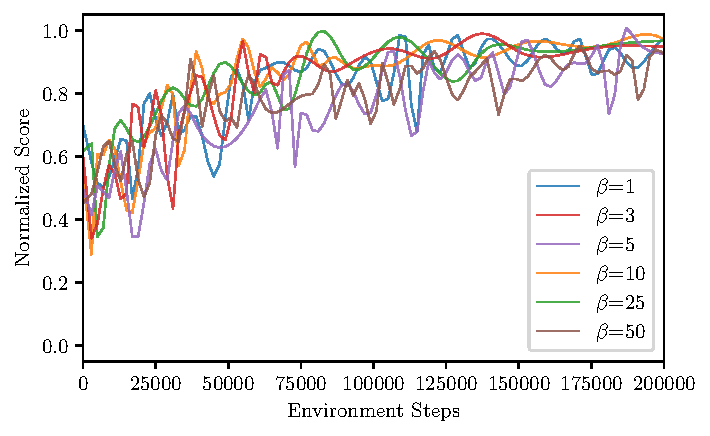
\includegraphics[width=0.45\textwidth]{figs-sample/iql-beta.pdf}}

\caption{\label{fig:beta_ablation}\footnotesize{\textbf{Abalation on IQL's online temperature values}: The change in the temperature $\beta$ used in online fine-tuning phase has little to no effect on the sample efficiency.}}
\end{center}
\vspace{-0.8cm}

\end{figure}

\begin{figure}[h]

\begin{center}
\centerline{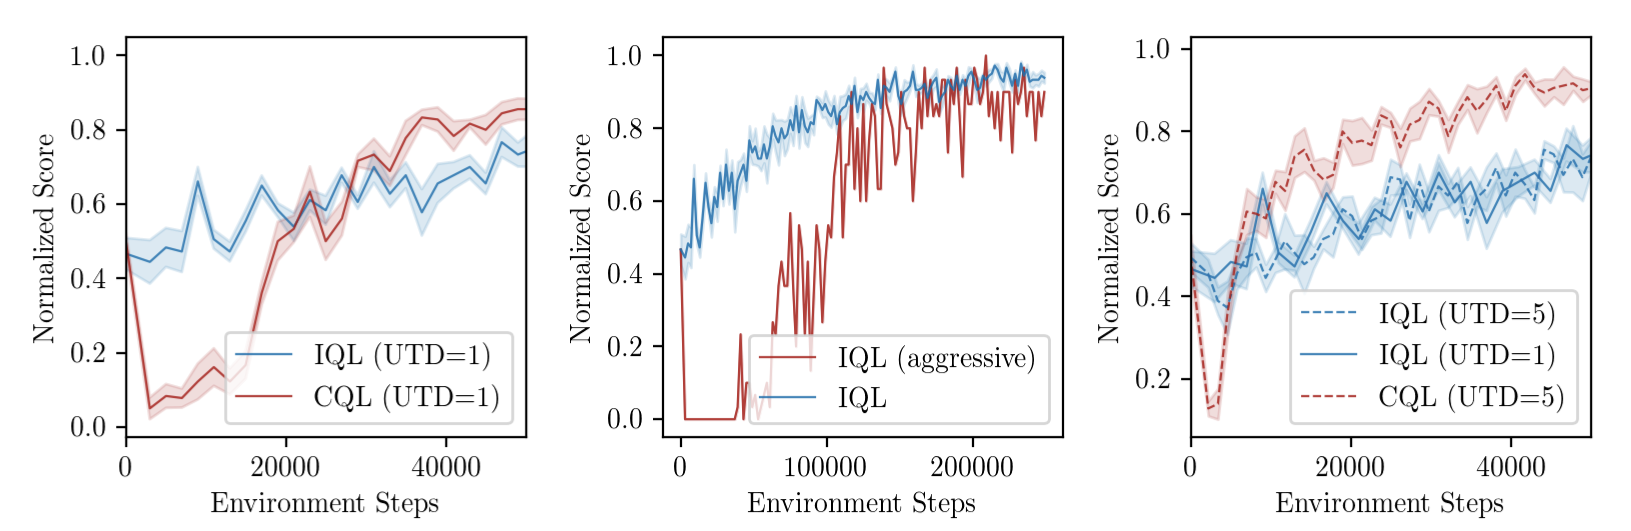
\includegraphics[width=0.8\textwidth]{figs-sample/iql-analysis-final.png}}

\caption{\label{fig:cql_iql_finetune_app}\footnotesize{\textbf{IQL and CQL:} Step 0 on the x-axis is the performance after offline pre-training. Observe while CQL suffers from initial policy unlearning, IQL improves slower throughout fine-tuning.}}

\end{center}
\vspace{-0.9cm}

\end{figure}


In this section, we aim to highlight some potential reasons behind the slow improvement of other methods in our empirical analysis experiment in Section~\ref{sec:empirical_analysis}, and specifically, we use IQL for the analysis. We first swept over the temperature $\beta$ values used in the online fine-tuning phase for IQL, which controls the constraint on how closely the learned policy should match the behavior policy. As shown in Figure~\ref{fig:beta_ablation}, the change in the temperature $\beta$ has little to no effect on the sample efficiency. Another natural hypothesis is that IQL improves slowly because we are not making enough updates per unit of data collected by the environment. To investigate this, we ran IQL with \textbf{(a)} five times as many gradient steps per step of data collection ($\text{UTD}=5$), and \textbf{(b)} with a more aggressive policy update. Observe in Figure~\ref{fig:cql_iql_finetune_app} that \textbf{(a)} does not improve the asymptotic performance of IQL, although it does improve CQL meaning that there is room for improvement on this task by making more gradient updates. Observe in Figure~\ref{fig:cql_iql_finetune_app} that \textbf{(b)} often induces policy unlearning, similar to the failure mode in CQL. These two observations together indicate that a policy constraint approach can slow down learning asymptotically, and we cannot increase the speed by making more aggressive updates as this causes the policy to find erroneously optimistic out-of-distribution actions, and unlearn the policy learned from offline data. 


\section{Impact of Estimation Errors in the Reference Value Function}
\label{app:nn_value_function}

\begin{wrapfigure}{r}{0.3\columnwidth}
\vspace{-0.9cm}
\begin{center}
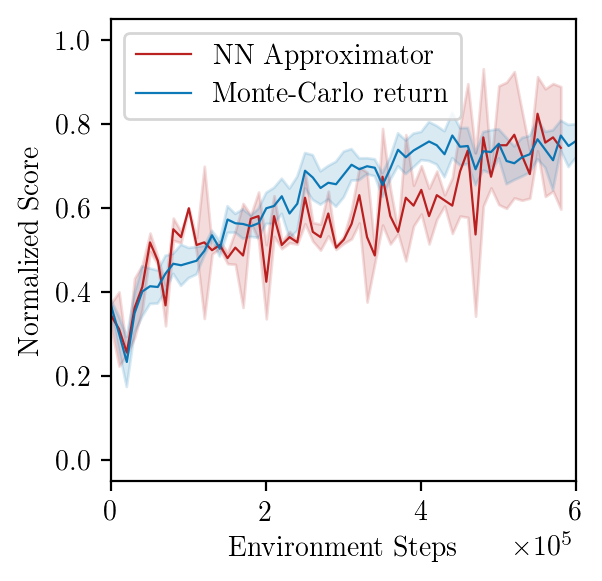
\includegraphics[width=0.9\linewidth]{figs-sample/kitchen-analysis.png}
\vspace{-0.2cm}
\caption{\footnotesize{The performance of \methodname\ using a neural net approximator for the reference value function is comparable to using the Monte-Carlo return.}}
\label{fig:kitchen-regress}
\vspace{-0.8cm}
\end{center}
\end{wrapfigure}

In our experiments, we compute the reference value functions using Monte-Carlo return estimates. However, this may not be available in all tasks. How does \methodname\ behave when reference value functions must be estimated using the offline dataset itself? To answer this, we ran an experiment on the \texttt{kitchen} domain, where instead of using an estimate for $Q^\mu$ based on the Monte-Carlo return, we train a neural network function approximator $Q^\mu_\theta$ to approximate $Q^\mu$ via supervised regression on to Monte-Carlo return, which is then utilized by \methodname. 
Observe in Figure \ref{fig:kitchen-regress}, that the performance of \methodname\ largely remains unaltered. This implies as long as we can obtain a reasonable function approximator to estimate the Q-function of the reference policy (in this case, the behavior policy), errors in the reference Q-function do not affect the performance of \methodname\ significantly.

\section{Initial Unlearning of CQL on Multiple Tasks}
\label{app:cql_dip_zoom_in}
\begin{figure}[b]
\vspace{-0.5cm}

\begin{center}    
{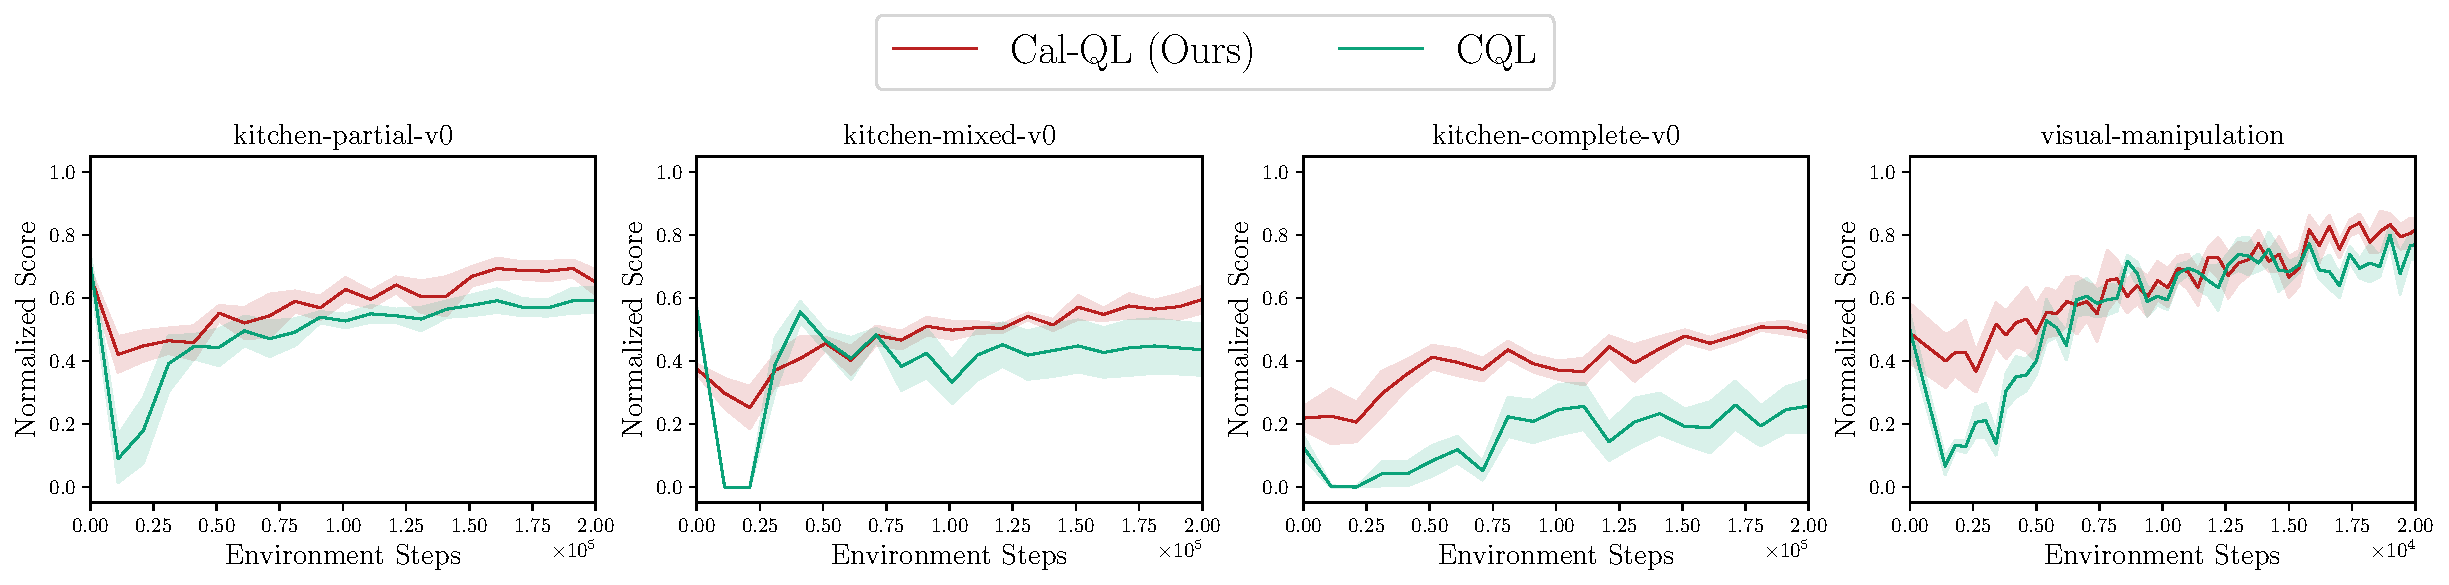
\includegraphics[clip,width=1\linewidth]{figs-sample/kitchen-cog-zoom-in.pdf}} {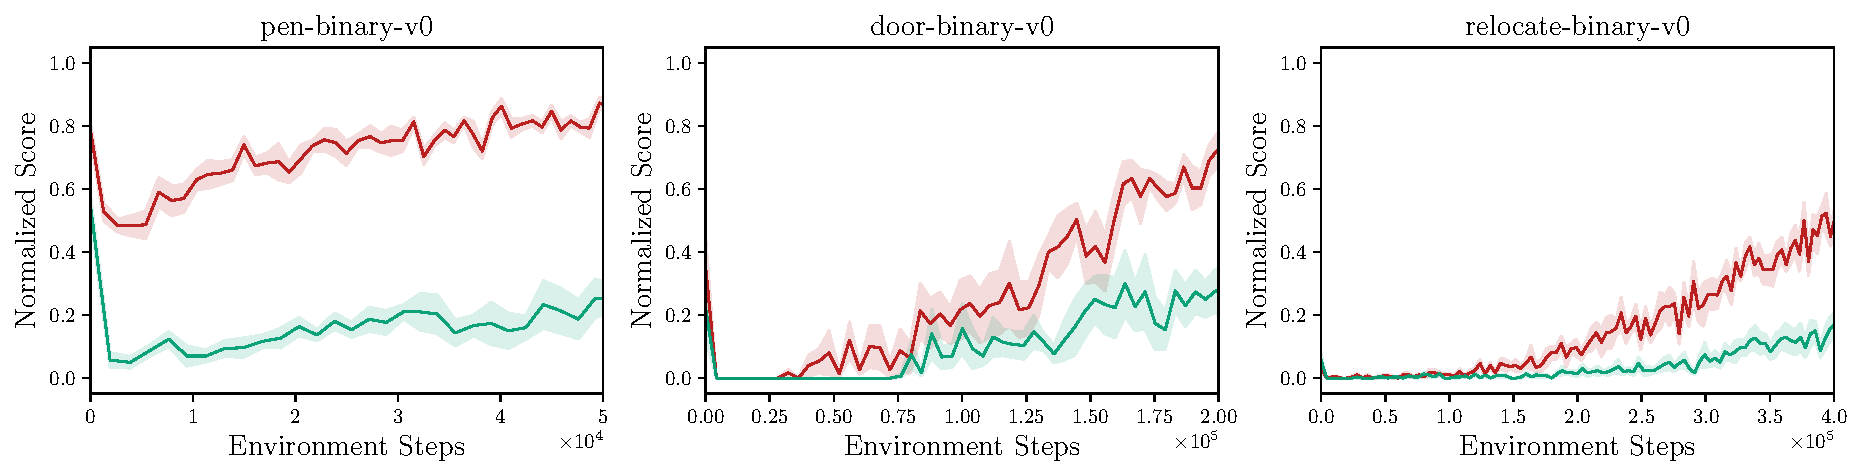
\includegraphics[clip,width=0.75\linewidth]{figs-sample/adroit-zoom-in.pdf}}
\end{center}
\vspace{-0.45cm}
\caption{\label{fig:dip_zoom} \footnotesize{While CQL experiences initial unlearning, \methodname\ effectively mitigates it and quickly recovers its performance.}}
\vspace{-0.6cm}
\end{figure}
In this section, we show the learning curves of CQL and \methodname\ from Figure~\ref{fig:all_tasks} and zoom in on the x-axis to provide a clearer visualization of CQL's initial unlearning in the Franka Kitchen, Adroit, and the visual-manipulation domains. As depicted in Figure~\ref{fig:dip_zoom}, it is evident across all tasks that while CQL experiences initial unlearning, \methodname\ can effectively mitigate it and quickly recovers its performance. Regarding the Antmaze domain, as we discussed in section~\ref{subsec:diagonistic}, CQL does not exhibit initial unlearning since the default dataset has a high coverage of data. However, we can observe a similar phenomenon if we narrow down the dataset distribution (as shown in Figure~\ref{fig:ant-narrow}).




\iffalse

\section{Discussion of Policy Unlearning in Fine-Tuning}

In this section, we provide another explanation for the performance drop shown in Figure~\ref{fig:cql_q_value} following the tabular setting. Specifically, in Section~\ref{subsec:reward-bias}, we show that running bellman iteration w.r.t. the CQL objective function~\eqref{eqn:cql_training} will converge to another Q-values w.r.t. a different (or biased) reward function $r^\pi_{\alpha,\beta}=r(\bs,\ba) - \alpha\brac{ \frac{\pi(\ba|\bs)}{\pi_\beta(\ba|\bs)} - 1 }$, where $\alpha$ is the regularizer of the CQL objective, and $\pi_\beta$ is the behavior policy. Note that this estimate only becomes unbiased when $\pi=\pi_\beta$.

In the fine-tuning phase, suppose we are using the CQL objective with another behavior policy $\pi_{\beta^\prime}$ and $\alpha^\prime$, then the Bellman operator will converge to a Q-value w.r.t. another (biased) reward function $r^\pi_{\alpha^\prime,\beta^\prime}=r(\bs,\ba) - \alpha^\prime\brac{ \frac{\pi(\ba|\bs)}{\pi_{\beta^\prime}(\ba|\bs)} - 1 }$. In Theorem~\ref{thm:mixing-dip-main}, we provide an if and only if condition under which the Q-values in the fine-tuning phase remain unchanged. But since the condition in Theorem~\ref{thm:mixing-dip-main} is generally hard to satisfy. Hence, it may lead to a performance difference gap in the fine-tuning phase in terms of the Q-values, as observed in Figure~\ref{fig:cql_q_value}.

\subsection{Bellman Consistency Equation of CQL}
 
\label{subsec:reward-bias}


To analyze policy unlearning with conservative methods at the beginning of online fine-tuning, we consider a tabular setting, where we are learning conservative value functions using a generic policy-iteration style offline RL method based on CQL~\citep{kumar2020conservative}. Our goal is to understand the differences in a policy obtained by running one round of policy improvement with and without additional online data. Key to our analysis is the Bellman backup induced by CQL (Equation~\ref{eqn:cql_training}):
\begin{align}
\label{eq:cql-bellman-consistency}
\footnotesize{
    Q^\pi(\bs, \ba) = \left(\mathcal{B}^\pi Q^\pi \right)(\bs, \ba) - \alpha \left[ \frac{\pi(\ba|\bs)}{\pi_\beta(\ba|\bs)} - 1 \right].}
\end{align}
By expanding $\mc B^\pi$, Equation~\ref{eq:cql-bellman-consistency} can also be interpreted as running standard Q-iteration in an MDP with a pessimistic reward function, which depends upon the learned policy $\pi$, the behavior policy $\pi_\beta$ induced by the dataset, and the coefficient $\alpha$ from Equation~\ref{eqn:cql_training}:
$r^\pi_{\alpha,\beta}(\bs,\ba) = r(\bs,\ba) - \alpha\brac{ \frac{\pi(\ba|\bs)}{\pi_\beta(\ba|\bs)} - 1 }$. This means that once online fine-tuning commences with a new regularizer $\alpha$, and a new behavior policy $\pi_{\beta^\prime}$ induced by online data added to the buffer, the pessimistic reward function $r^\pi_{\alpha,\beta}$ may {\em bias towards} $r^\pi_{\alpha^\prime,\beta^\prime}$. Hence, the policy improvement on the resulting Q-function with the online data may simply not lead to any policy improvement on the ground-truth reward function. We will first provide a condition such that the pessimistic Q-function is invariant to such reward bias during the online fine-tuning, and then show how our approach alleviates the reward bias.


\paragraph{Performance difference during fine-tuning.} 
Consider the fixed points from solving Equation~\ref{eq:cql-bellman-consistency} w.r.t. the biased rewards $r^\pi_{\alpha,\beta}$ and $r^\pi_{\alpha^\prime,\beta^\prime}$, Theorem~\ref{thm:mixing-dip-main} provides a necessary and sufficient condition for the fixed points to be invariant to reward bias.
\begin{theorem}[Invariant Conservative Q Functions]
\label{thm:mixing-dip-main}
Let $Q$ and $Q^\prime$ denote the conservative value function from solving the fixed point Equation~\ref{eq:cql-bellman-consistency}
with regularizers $\alpha,\alpha^\prime$ and behavior policies $\pi_\beta,\pi_{\beta^\prime}$ respectively. Then for a given policy $\pi$, $Q(s,a) = Q^\prime(s,a),\forall s\in \mc S$ if and only if
\begin{equation}
    \label{eq:inv-cond}
    \footnotesize{
    \frac{\alpha}{\pi_\beta(a|s)}-\frac{\alpha^\prime}{\pi_{\beta^\prime}(a|s)}=\frac{\alpha-\alpha^\prime}{\pi(a|s)},\;\forall (s,a)\in \mc S\times \mc A.}
\end{equation}
\end{theorem}
The proof of Theorem~\ref{thm:mixing-dip-main} is provided in Appendix~\ref{appendix:proof:mixing-dip-main}. Theorem~\ref{thm:mixing-dip-main} implies that one shall expect a performance change in the fine-tuning phase, whenever Equation~\ref{eq:inv-cond} becomes invalid. Unfortunately, Equation~\ref{eq:inv-cond} is generally hard to enforce in practice since the new behavior policy $\pi_{\beta^\prime}$ and the updated policy $\pi$ may be intractable, as suggested by the performance dip in Section~\ref{sec:empirical_analysis}.

\paragraph{Preventing unlearning via calibration.}
Since the standard CQL training objective suffers from reward bias, which may continue to deteriorate during fine-tuning. The next corollary provides a condition under which $r^\pi_{\alpha,\beta}(s,a)$ becomes unbiased.
\begin{corollary}
\label{coro:calibration-prevent-dip}
The reward function $r^\pi_{\alpha,\beta}(s,a)$ induced by the CQL training (Equation~\ref{eq:cql-bellman-consistency}) becomes unbiased when $\pi = \pi_\beta$: $r^{\pi_\beta}_{\alpha,\beta}(s,a)=r(s,a),\forall (s,a)\in \mc S\times \mc A.$
\end{corollary}
The proof of Corollary~\ref{coro:calibration-prevent-dip} is straight forward as substituting $\pi = \pi_\beta$ will set $\brac{\frac{\pi(a|s)}{\pi_\beta(a|s)}-1}=0$, which makes Equation~\ref{eq:cql-bellman-consistency} become a Bellman backup w.r.t. the original reward $r(s,a)$. Corollary~\ref{coro:calibration-prevent-dip} implies that the CQL-induced Bellman backup (Equation~\ref{eqn:cql_training}) becomes unbiased when the updating policy equals the behavior policy. Hence, if one aims at using a neural network $Q_\theta$ to approximate the CQL Bellman backup w.r.t. behavior policy $\pi_\beta$, one shall consider using $Q^{\pi_\beta}(s,a)$ to calibrate the bias. This empirically implies that we shall use $Q^{\pi_\beta}(s,a)$ and $Q^{\pi_{\beta^\prime}}(s,a)$ to calibrate the $Q_\theta$ during offline and online phase, as we have presented in Definition~\ref{cond:calibration} and Section~\ref{sec:empirical-method}.

\subsection{Notations}
In this subsection, we provide the notations for deriving the Bellman Consistency Equation of the conservative Bellman Consistency equation (CQL Objective)~\eqref{eq:cql-bellman-consistency}. Our matrix notation follows~\cite{li2020breaking}. 
\begin{itemize}
    \item We consider the infinite horizon tabular setting where $\mc S$ and $\mc A$ are discrete and finite, $\gamma \in (0,1)$ is a discount factor and $r:\mc S\times \mc A \mapsto[0,1]$ is the reward function;
    \item The value function $V^\pi(s)$ of a state w.r.t. policy $\pi$ is defined as 
    \begin{equation}
        V^\pi(s) := \bb E\brac{\sum_{t=0}^\infty \gamma^t r(s^t,a^t)|s^0=s},\;\forall s \in \mc S;
    \end{equation}
    \item The Q function $Q^\pi(s,a)$ of a state action pair $(s,a)$ w.r.t. a policy $\pi$ is defined by
    \begin{equation}
        Q^\pi(s,a):=\bb E\brac{\sum_{t=0}^\infty\gamma^t r(s^t,a^t)|s^0=s,a^0=a}\forall (s,a)\in \mc S\times \mc A;
    \end{equation}
    \item $\mb P\in \bb R^{|\mc S||\mc A|\times |\mc S|}$ is a matrix of the transition kernel $P$;
    \item $\mb P^\pi\in\bb R^{|\mc S||\mc A|\times |\mc S||\mc A|}$ and  $\mb P_\pi\in\bb R^{|\mc S|\times |\mc S|}$ two square probability transition matrices induced by the policy $\pi$ over the state-action pair and the states respectively, defined by
    \begin{equation}
        \mb P^\pi := \mb P \mb \Pi^\pi,\quad \mb P_\pi := \mb \Pi^\pi\mb P;
    \end{equation}
    \item $\mb \Pi^\pi\in \{0,1\}^{|\mc S|\times |\mc S||\mc A|}$ is a projection matrix:
    \begin{equation}
        \mb \Pi^\pi = 
        \begin{pmatrix}
            \mb e^\top_{\pi(1)} & & & \\
             & \mb e^\top_{\pi(2)} & & \\
             & & \ddots & \\
             & & & \mb e^\top_{\pi(|\mc S|)}.
        \end{pmatrix}
    \end{equation}
    \item $\mb r\in \bb R^{|\mc S||\mc A|}$ is the reward function
    \item $\mb r^\pi \in \bb R^{|\mc S|}$ is the reward function following policy $\pi$, simply we have $\mb r^\pi = \mb \Pi^\pi\mb r$.
\end{itemize}
\subsection{Derivations of Conservative Bellman Consistency Equation~\ref{eq:cql-bellman-consistency}}
$\forall (s,a)\in \mc S\times \mc A$, the tabular CQL optimization (Equation~\ref{eqn:cql_training}) aims at solving the following optimization problem:
\label{appendix:cql-critical-point}
\begin{equation}
    \begin{split}
        \min_{Q(s,a)} \alpha \brac{ \underset{s\sim \mc D,a\sim \pi}{\bb E}Q(s,a)-\underset{(s,a)\sim \mc D,a\sim \pi_\beta}{\bb E}Q(s,a)}+\frac{1}{2}\underset{s\sim \mc D,a\sim \pi_\beta}{\bb E}\brac{\paren{Q(s,a)-\mc B^\pi Q(s,a)}^2}.
    \end{split}
\end{equation}
If we rewrite $x = Q(s,a)$ and define function $f(x)$ as
\begin{equation}
    f(x) := \alpha \brac{ \underset{s\sim \mc D,a\sim \pi}{\bb E}x-\underset{(s,a)\sim \mc D,a\sim \pi_\beta}{\bb E}x}+\frac{1}{2}\underset{s\sim \mc D,a\sim \pi_\beta}{\bb E}\brac{\paren{x-\mc B^\pi x}^2},
\end{equation}
setting $f^\prime(x) = 0$ yields
\begin{equation}
    \alpha \paren{\pi(a|s) - \pi_\beta(a|s)} + \pi_\beta(x - \mc B^\pi x) = 0,
\end{equation}
which leads to 
\begin{equation}
    x = \mc B^\pi x - \alpha\brac{\frac{\pi(a|s)}{\pi_\beta(a|s)}-1}.
\end{equation}

\subsection{Conservative Bellman Consistency Equations}
\paragraph{Q Functions.}
Considering the matrix form and point-wise Bellman consistency equation, we have
\begin{align}
    \mb Q^\pi &= \mb r + \gamma \mb P^\pi \mb Q^\pi\implies \mb Q^\pi = \paren{\mb I - \gamma \mb P^\pi}^{-1}\mb r\\
    Q^\pi(s,a) &= r(s,a) + \gamma \brac{\mb P^\pi \mb Q^\pi}_{(s,a)},\;\forall (s,a)\in \mc S\times \mc A,
\end{align}
where we use $\brac{\mb P^\pi \mb Q^\pi}_{(s,a)}$ to denote the entries $(s,a)^\text{th}$ of the matrix $\mb P^\pi \mb Q^\pi$.
Now recall the point-wise Bellman consistency equation of the CQL objective~\eqref{eq:cql-bellman-consistency}, we also have the following point-wise consistency equation:
\begin{align}
    Q_{\alpha,\beta}^\pi(s,a) &= r(s,a) + \gamma \brac{\mb P^\pi \mb Q_{\alpha,\beta}^\pi}_{(s,a)} - \alpha\brac{\frac{\pi(a|s)}{\pi_\beta(a|s)}-1},\;\forall (s,a)\in \mc S\times \mc A,\\
    &= r_{\alpha,\beta} + \gamma \brac{\mb P^\pi \mb Q^\pi}_{(s,a)},
\end{align}
where 
\begin{equation}
    \label{eq:new-bellman-reward-cql}
    r^\pi_{\alpha,\beta}(s,a) := r(s,a) - \alpha\brac{\frac{\pi(a|s)}{\pi_\beta(a|s)}-1},\;\forall (s,a)\in \mc S\times \mc A.
\end{equation}
Hence, we can similarly have the bellman-consistency equation of CQL in matrix form:
\begin{equation}
    \mb Q_{\alpha,\beta} = \mb r_{\alpha,\beta} + \gamma \mb P^\pi \mb Q^\pi_{\alpha,\beta} \implies \mb Q^\pi_{\alpha,\beta}=\paren{\mb I - \gamma \mb P^\pi}^{-1}\mb r_{\alpha,\beta}.
\end{equation}
\paragraph{Value Functions.} Now considering the Bellman Consistency equation of the Value function, we have
\begin{align}
    \mb V^\pi &= \mb r^\pi + \gamma \mb P_\pi \mb V^\pi\implies\mb V^\pi = (\mb I - \gamma \mb P_\pi)^{-1}\mb r^\pi\\
    \mb V_{\alpha,\beta}^{\pi} &= \mb r^\pi_{\alpha,\beta} + \gamma \mb P_\pi \implies \mb V_{\alpha,\beta}^\pi = (\mb I - \gamma \mb P_\pi)^{-1}\mb r_{\alpha,\beta}^\pi.
\end{align}


\paragraph{Summary.} In summary, for a given reward function $\mb r$, a fixed policy $\pi$, a behavior policy $\pi_\beta$, and a fixed constant $\alpha$, the {\em policy evaluation} for CQL satisfies:
\begin{equation}
    \label{eq:cql-consistency-equation}
    \begin{split}
         \mb V_{\alpha,\beta}^{\pi} & = (\mb I - \gamma \mb P_\pi)^{-1}\mb r_{\alpha,\beta}^\pi = (\mb I - \gamma \mb P_\pi)^{-1}\mb \Pi^\pi\brac{\mb r - \alpha\paren{\mb\pi/\mb\pi_\beta-\mb 1}} \\
         \mb Q^\pi_{\alpha,\beta}&=\paren{\mb I - \gamma \mb P^\pi}^{-1}\mb r_{\alpha,\beta}=\paren{\mb I - \gamma \mb P^\pi}^{-1}\brac{\mb r - \alpha\paren{\mb\pi/\mb\pi_\beta-\mb 1}}.
    \end{split}
\end{equation}
where $\pi/\pi_\beta\in \bb R^{|\mc S|\times |\mc A|}$ is a vector whose $(s,a)$ entry denotes $\pi(a|s)/\pi_\beta(a|s)$ and $\mb 1=\{1,1,\dots,1\}^\top\in \bb R^{|\mc S||\mc A|}$.

\subsection{Proof of Theorem~\ref{thm:mixing-dip-main}}
\label{appendix:proof:mixing-dip-main}
\begin{theorem}[Invariant Conservative Q Functions]
Let $Q^\pi_{\alpha,\beta}$ and $Q^\pi_{\alpha^\prime,\beta^\prime}$ denote the conservative value function from solving the conservative bellman consistency equation (Equation~\ref{eq:cql-bellman-consistency} and~\ref{eq:cql-consistency-equation}) with regularizers $\alpha,\alpha^\prime$ and behavior policies $\pi_\beta,\pi_{\beta^\prime}$ respectively. Then for a given policy $\pi$, $Q^\pi_{\alpha,\beta}(s) = Q^\pi_{\alpha^\prime,\beta^\prime}(s),\forall s\in \mc S$ if and only if
\begin{equation}
    \frac{\alpha}{\pi_\beta(a|s)}-\frac{\alpha^\prime}{\pi_{\beta^\prime}(a|s)}=\frac{\alpha-\alpha^\prime}{\pi(a|s)},\;\forall (s,a)\in \mc S\times \mc A.
\end{equation}
\end{theorem}
\begin{proof}
\label{proof:mixing-dip-main}
% Now consider we updated our behavior policy by
% \begin{equation}
%     \mb \pi_{\beta^\prime} = \delta \mb \pi_{\beta} + (1-\delta) \mb \pi_\mr{on}, 
% \end{equation}
% where
% \begin{equation}
%     \pi_{\beta^\prime}(a|s) = 
%     \begin{cases}
%         \pi_\beta(a|s),\;&\text{with probability } \delta,\\
%         \pi_\mr{on}(a|s),\;&\text{with probability } 1-\delta.\\
%     \end{cases}
% \end{equation}
By the conservative Bellman Consistency~\eqref{eq:cql-consistency-equation}, we know that changing a behavior policy from $\pi_\beta$ to $\pi_{\beta^\prime}$ and changing the regularize from $\alpha$ to $\alpha^\prime$, we have
\begin{equation}
    \begin{split}
        \mb Q_{\alpha,\beta}^{\pi} - \mb Q_{\alpha^\prime,\beta^\prime}^{\pi} & = (\mb I - \gamma \mb P^\pi)^{-1}(\mb r_{\alpha,\beta}^\pi-\mb r_{\alpha^\prime,\beta^\prime}^\pi)  \\
        & =(\mb I - \gamma \mb P^\pi)^{-1}\brac{\alpha\paren{\frac{\mb\pi}{\mb\pi_\beta}-\mb 1}-\alpha^\prime\paren{\frac{\mb\pi}{\mb\pi_{\beta^\prime}}-\mb 1}}.
    \end{split} 
\end{equation}
Since $(\mb I - \gamma \mb P)^{-1}$ is a square and full rank matrix, $ \mb Q_{\alpha,\beta}^{\pi} - \mb Q_{\alpha^\prime,\beta^\prime}^{\pi} = \mb 0$ holds if and only if
\begin{equation}
    \alpha\paren{\frac{\mb\pi}{\mb\pi_\beta}-\mb 1}-\alpha^\prime\paren{\frac{\mb\pi}{\mb\pi_{\beta^\prime}}-\mb 1} = \mb 0\implies \frac{\alpha}{\pi_\beta(a|s)}-\frac{\alpha^\prime}{\pi_{\beta^\prime}(a|s)}=\frac{\alpha-\alpha^\prime}{\pi(a|s)},\;\forall (s,a)\in \mc S\times \mc A,
\end{equation}
which finishes the proof.
\end{proof}

\fi
